%%%%%%%%%%%%%%%%%%%%%%%%%%%%%%%%%%%%%%%%%%%%%%%%%%%%%%%%%%%%%%%%%%%%%%%%%%%%%%%%%%%%%%
% Modelo de Proposta de TCCs de Especialização
% Preparado por Leandro Krug Wives a partir do 
% pacote ii-ufrgs.zip disponivel em http://www.inf.ufrgs.br/utug
%%%%%%%%%%%%%%%%%%%%%%%%%%%%%%%%%%%%%%%%%%%%%%%%%%%%%%%%%%%%%%%%%%%%%%%%%%%%%%%%%%%%%%

%%%%%%%%%%%%%%%%%%%%%%%%%%%%%%%%%%%%%%%%%%%%%%%%%%%%%%%%%%%%%%%%%%%%%%%%%%%%%%%%%%%%%%
% Definição do tipo / classe de documento e estilo usado
%%%%%%%%%%%%%%%%%%%%%%%%%%%%%%%%%%%%%%%%%%%%%%%%%%%%%%%%%%%%%%%%%%%%%%%%%%%%%%%%%%%%%%
%
\documentclass[prop-esp]{iiufrgs}

%%%%%%%%%%%%%%%%%%%%%%%%%%%%%%%%%%%%%%%%%%%%%%%%%%%%%%%%%%%%%%%%%%%%%%%%%%%%%%%%%%%%%%
% Importação de pacotes
%%%%%%%%%%%%%%%%%%%%%%%%%%%%%%%%%%%%%%%%%%%%%%%%%%%%%%%%%%%%%%%%%%%%%%%%%%%%%%%%%%%%%%
% (a A seguir podem ser importados os pacotes necessários para o documento, de acordo 
% com a necessidade)
%
\usepackage[brazilian]{babel}	    % para texto escrito em pt-br
\usepackage[utf8]{inputenc}         % pacote para acentuação
\usepackage{graphicx}         	    % pacote para importar figuras
\usepackage[T1]{fontenc}            % pacote para conj. de caracteres correto
\usepackage{times}                  % pacote para usar fonte Adobe Times
\usepackage{enumerate}              % para lista de itens com letras
\usepackage{breakcites}
\usepackage{titlesec}
\usepackage{enumitem}
\usepackage{titletoc}               
%\usepackage{fixltx2e}              % para subscript
%\usepackage{amsmath}               % para \epsilon e matemática
%\usepackage{amsfonts}
%\usepackage{listings}			    % para listagens de código-fonte
%\usepackage{color}				    % para imagens e outras coisas coloridas
%\usepackage{mathptmx}              % p/ usar fonte Adobe Times nas formulas matematicas
%\usepackage{url}                   % para formatar URLs
%\usepackage[table,xcdraw]{xcolor}  % para tabelas coloridas
%\usepackage{longtable}             % para tabelas compridas (mais de uma página)
%\usepackage{float}
%\usepackage{booktabs}
%\usepackage{tabularx}
%\usepackage[breaklinks]{hyperref}
%\usepackage{caption} 

\usepackage[alf,abnt-emphasize=bf]{abntex2cite}	% pacote para usar citações abnt


%%%%%%%%%%%%%%%%%%%%%%%%%%%%%%%%%%%%%%%%%%%%%%%%%%%%%%%%%%%%%%%%%%%%%%%%%%%%%%%%%%%%%%
% Macros, ajustes e definições
%%%%%%%%%%%%%%%%%%%%%%%%%%%%%%%%%%%%%%%%%%%%%%%%%%%%%%%%%%%%%%%%%%%%%%%%%%%%%%%%%%%%%%
%

% define estilo de parágrafo para citação longa direta:
\newenvironment{citacao}{
    %\singlespacing
    %\footnotesize
    \small
    \begin{list}{}{
        \setlength{\leftmargin}{4.0cm}
        \setstretch{1}
        \setlength{\topsep}{1.2cm}
        \setlength{\listparindent}{\parindent}
    }
    \item[]}{\end{list}
}

% adiciona a fonte em figuras e tabelas
\newcommand{\fonte}[1]{\\Fonte: {#1}}

% Ative o seguinte caso alguma nota de rodapé fique muito longa e quebre entre múltiplas
% páginas
%\interfootnotelinepenalty=10000

%%%%%%%%%%%%%%%%%%%%%%%%%%%%%%%%%%%%%%%%%%%%%%%%%%%%%%%%%%%%%%%%%%%%%%%%%%%%%%%%%%%%%%
% Informações gerais                                   
%%%%%%%%%%%%%%%%%%%%%%%%%%%%%%%%%%%%%%%%%%%%%%%%%%%%%%%%%%%%%%%%%%%%%%%%%%%%%%%%%%%%%%

% título
\title{Otimizando StarVZ para carga de grandes volumes de dados} 

% autor
\author{Miyazaki}{Alexandre K. S.}

% orientador
\advisor[Prof.~Dr.]{Schnorr}{Lucas M.} 

% coorientador (se houver)
%\coadvisor[Prof.~Dr.]{Sobrenome}{Nome}

% local da realização (defesa) do trabalho 
\location{Porto Alegre}{RS} 

% data da realização (defesa) do trabalho (mês e ano)
\date{05}{2019}

% nome do curso 
\course{Curso de Especialização em Big Data \& Data Science}

% Palavras chave
\keyword{Palavra-chave1}
\keyword{Palavra-chave2}
\keyword{Palavra-chave3}

%%%%%%%%%%%%%%%%%%%%%%%%%%%%%%%%%%%%%%%%%%%%%%%%%%%%%%%%%%%%%%%%%%%%%%%%%%%%%%%%%%%%%%
% Início do documento e elementos pré-textuais
%%%%%%%%%%%%%%%%%%%%%%%%%%%%%%%%%%%%%%%%%%%%%%%%%%%%%%%%%%%%%%%%%%%%%%%%%%%%%%%%%%%%%%

% Declara início do documento
\begin{document}

% inclui folha de rosto 
\maketitle      

\selectlanguage{brazilian}


%%%%%%%%%%%%%%%%%%%%%%%%%%%%%%%%%%%%%%%%%%%%%%%%%%%%%%%%%%%%%%%%%%%%%%%%%%%%%%%%%%%%%
% Introdução
%
\chapter{Introdução} \label{intro}

A quantidade de dados gerados em todo o mundo diariamente é surpreendente. De acordo com \citet{ref:data_minute2}, há uma estimativa
que em 2020 cada pessoa deve gerar em média 1,7MB de dados por dia. Estes frequentemente precisam ser processados para ter algum valor,
o que implica em uma constante necessidade por sistemas computacionais mais poderosos.

Plataformas de HPC (\emph{High-Performance Computing}) evoluíram para utilizar algumas tecnologias, como processadores multicore e GPUs (\emph{Graphics processing units}, comumente referenciadas como \emph{accelerators}), inserindo uma variabilidade de recursos nessas plataformas. Com a evolução do Hardware, a abordagem de desenvolvimento de aplicações de HPC tradicional, chamada de \emph{Bulk-synchronous parallel} (BSP) tornou-se obsoleta. Esta espera que os recursos de computação sejam homogêneos (nós idênticos, conectados por links estáveis e de alta vazão) e portanto, é incapaz de utilizar a heterogeneidade do ambiente ao seu favor. 

Uma abordagem que está sendo utilizada é desenvolver a aplicação em alto nível, descrevendo as computações como um \emph{Directed Acyclic Graph} (DAG) de tarefas. Tal abordagem é implementada por múltiplos modelos de programação: OpenMP 4 \cite{ref:openmp4}, StarPU \cite{ref:starpu}, OmpSs \cite{ref:ompss}, ParSEC \cite{ref:parsec}, etc. 

Nesses modelos de programação \emph{task-based}, a responsabilidade de escalonar e executar a aplicação de forma performática é atribuída para outra camada de software, denominada \emph{runtime}. Ferramentas de análise de \emph{traces}, que antes auxiliavam o desenvolvedor da aplicação a fazer otimizações, como Paraver \cite{ref:paraver} e Vampir \cite{ref:vampir} não são eficazes ao analisar aplicações baseadas em tarefas.

Com essa motivação, foi desenvolvido um \emph{framework} denominado StarVZ \cite{ref:starvz}, cujo objetivo é fornecer uma visualização de traces mais elaborada, provendo facilidade no entendimento e identificação de problemas de performance sutis, que dificilmente seriam identificados com abordagens clássicas. Esse \emph{framework} foi desenvolvido combinando \emph{pj\_dump},  a linguagem R \cite{ref:rlanguage} e algumas bibliotecas expressivas dessa linguagem (\emph{ggplot2} \cite{ref:ggplot2}, \emph{lpSolve} \cite{ref:lpsolve} e \emph{tidyverse} \cite{ref:tidyverse}), Org-mode \cite{ref:org-mode} e \emph{plotly} para análise de traces gerados pelo modelo de programação StarPU.

Em alguns estudos de caso onde o StarVZ foi utilizado, de fato identificaram-se problemas de performance do StarPU.
A primeira fase do \emph{framework} (pré-processamento de dados) em um dos experimentos levou cerca de 32 minutos para processar 18 GB de dados. Essa fase deve ser melhorada pois a tendência é que aplicações gerem \emph{traces} cada vez mais volumosos, tendo em vista que vez sua tendência é aumentar ou em recursos ou em dimensão (mais dados e/ou processamentos maiores).

Este documento consiste em uma proposta de trabalho de conclusão de curso da Especialização em Big Data \& Data Science. As próximas Seções estão organizadas da seguinte forma:
\begin{itemize}
    \item a Seção \ref{lbl:fundamentacao} descreve a fundamentação teórica;
    \item a Seção \ref{lbl:objetivos} mostra os objetivos a serem alcançados;
    \item a Seção \ref{lbl:metodologia} expõe em alto nível como os objetivos pretendem ser alcançados; e
    \item a Seção \ref{lbl:cronog} apresenta o cronograma previsto para a execução do trabalho.
\end{itemize}


%%%%%%%%%%%%%%%%%%%%%%%%%%%%%%%%%%%%%%%%%%%%%%%%%%%%%%%%%%%%%%%%%%%%%%%%%%%%%%%%%%%%%
% FUNDAMENTAÇÃO TEÓRICA
%
\chapter{Fundamentação Teórica} \label{lbl:fundamentacao}

Nesta seção, serão apresentados os trabalhos relacionados. Eles foram agrupados em dois grupos, buscando melhor organização do trabalho:

\begin{itemize}
\item Ferramentas de visualização Clássicas - oferecem visualização de \emph{traces} de aplicações desenvolvidas no modelo BSP;
\item Ferramentas de visualização orientadas a tarefas - oferecem visualização de traces de aplicações desenvolvidas no modelo orientado a tarefas.
\end{itemize}

Nas próximas subseções, serão detalhados os trabalhos de cada um desses grupos.

\subsection*{Ferramentas de visualização Clássicas}

Essas ferramentas possuem o objetivo de prover visualizações de traces para aplicações de HPC tradicionais. Estas eram desenvolvidas
seguindo o modelo que consiste em uma série de \emph{supersteps} (computações, comunicações, sincronizações), executadas com a premissa de ter-se um ambiente homogêneo, denominado \emph{Bulk-Synchronous Parallel}. Como esta abordagem  dominou o cenário HPC durante muito tempo, suas necessidades
balizaram o desenvolvimento da maior parte das ferramentas de análise de desempenho.

\subsubsection*{ViTE}
ViTE \cite{ref:vite} é uma ferramenta de visualização de \emph{traces} open-source. Para o processamento de grandes entradas ele conta com aceleração de Hardware e OpenGL. Suas entradas são arquivos na linguagem Paje \cite{ref:paje}.

Essa ferramenta exibe os recursos de forma hierárquica, onde oferece a visualização das tarefas (eixo vertical) em função de tempo (eixo horizontal), similar a um Gantt. Na análise de aplicações distribuídas, também é possível incluir indicadores de transferências de dados.

\subsubsection*{Paraver}
Paraver \cite{ref:paraver} também objetiva a visualização e análise de \emph{traces} de execução. Ela conta com uma agregação de dados, definida pelo
usuário via arquivo de configuração, para conseguir exibir entradas volumosas. Suas entradas são greradas por vários modelos de programação, sendo gerados pela ferramenta Extrae.

\subsubsection*{Vampir}
Vampir \cite{ref:vampir} é uma ferramenta proprietária de código fechado para fins de análise de \emph{traces}. Ela traz uma abordagem de cliente-servidor, onde o servidor pode ser executado no hardware de experimentação e o cliente é o computador do usuário.

Suas entradas são arquivos OTF2 (Open Trace Format, version 2) \cite{ref:otf2}. Ele fornece múltiplas visualizações como gráficos de espaço-tempo e estatísticas de execução.

\subsubsection*{Ravel}
O objetivo da ferramenta Ravel \cite{ref:ravel} também é a visualização de \emph{traces}. Suas entradas são em formato OTF \emph{Open Trace Format} e sua diferença em relação aos demais é que ele mostra as linhas de tempo lógicas, fornecendo uma estruturação para melhor entendimento de operações.

\subsubsection*{FrameSoc e Ocelotl}

FrameSoc \cite{ref:framesoc} é uma ferramenta de análise de performance, capaz de lidar com grandes volumes de dados. Como entrada, ela suporta diversos
formatos como Pajé, CTF, Paraver e OTF2. Além dos dados de \emph{trace}, é possível armazenar informações como metadados e anotações. A ferramenta converte tudo para um modelo de dados genérico e armazena em uma base de dados relacional.

Para visualizar grandes volumes de dados, a ferramenta baseia-se no Ocelotl \cite{ref:ocelotl}. Esse módulo possui um arquivo de configuração parametrizável pelo usuário, que gerencia uma agregação de espaçotemporal dados.

\subsection*{Ferramentas de visualização orientadas a tarefas}

Como os recursos e o custo de execução de tarefas não são constantes no modelo \emph{task-based}, é necessário representações diferentes para
possibilitar uma análise de performance nesses ambientes. O desenvolvimento do \emph{framework} StarVZ \cite{ref:starvz} foi motivado pela carência
de ferramentas maduras para a visualização de \emph{traces} com o objetivo de identificação de melhorias de performance. Antes de seu desenvolvimento existiam algumas ferramentas, todavia, elas não forneciam dados suficientes para identificar otimizações de forma eficiente.

\subsubsection*{DAGViz}

DAGViz \cite{ref:dagviz} é composto por dois passos: 

\begin{enumerate}
    \item extração do DAG dos arquivos de uma execução paralela;
    \item visualização hierárquica do DAG.
\end{enumerate}

Essa ferramenta traz uma visualização diferente do modelo BSP, exibindo as tarefas como um grafo hierárquico. Nele, o analista pode colapsar e expandir os grupos de tarefas. Dados de tempo de execução não são tratados pela ferramenta.

\subsubsection*{Traces de execução com dependências de tarefas}

A ferramenta desenvolvida por \citet{ref:visuexecdep} traz um gráfico no estilo espaço-tempo (Gantt). Há algumas outras funcionalidades como a identificação de dependências de tarefas (apenas o primeiro nível) a medida que o usuário passa o mouse sobre as caixas que representam as tarefas.

Como entradas, são utilizados a representação do DAG e os \emph{traces} de execução. Essa ferramenta é desenvolvida para o especificamente para o \emph{runtime} PaRSEC.

\subsubsection*{Temanejo}

Temanejo \cite{ref:temanejo} é um \emph{debugger} para o modelo de programação baseado em tarefas, onde o analista visualiza um DAG. Ele suporta grande parte dos 
\emph{runtimes} de execução de aplicações baseadas em tarefas, como OmpSs, StarPU e PaRSEC. As funcionalidades dessa ferramenta são focadas em depuração, permitindo que o usuário possa identificar e consertar parâmetros e dependências de tarefas.

\subsubsection*{Delay Spotter}

Delay Spotter \cite{ref:delayspotter} é uma ferramenta, construída sobre o DAGViz, que possibilita a identificação de atrasos em \emph{runtimes}.
Ela divide os estados dos \emph{workers} em três categorias, permitindo a identificação de delays decorrentes de problemas de escalonamento.
Como em ambientes heterogêneos com tarefas variadas, a presença de \emph{delays} faz parte da execução das aplicações, essa ferramenta é pouco efetiva.

\subsubsection*{TaskInsight}

TaskInsight \cite{ref:taskinsight} é uma ferramenta que objetiva identificar o comportamento de memória e seu impacto na execução de tarefas. 
Apesar de prover algumas estatísticas e possibilitar algumas identificações de anomalias, apenas essa análise não é o suficiente para
identificar a maioria dos pontos de otimização de aplicações \emph{task-based}.

\subsubsection*{StarVZ}

Framework que é objeto deste trabalho, o StarVZ \cite{ref:starvz} possui a visualização de dados mais avançada dentre as ferramentas citadas.
Construído com uma abordagem de \emph{script}, ela possui um grande poder de customização e, por isso, é difícil enumerar o que a ferramenta fornece.
No trabalho de \citet{ref:starvz}, podemos visualizar diversos gráficos gerados de apenas uma execução de aplicação:

\begin{itemize}
    \item gráfico com comportamento de tarefas;
    \item gráfico com a quantidade de tarefas submetidas;
    \item o comportamento do \emph{runtime}, com os estados dos workers StarPU;
    \item a quantidade de tarefas prontas;
    \item taxa de GFlops do ambiente;
    \item tráfego de dados entre a memória das GPUs;
    \item transferências de rede MPI;
    \item número de operações MPI concorrentes.
\end{itemize}

Ele é composto por dois passos sendo o primeiro, executado em um servidor e cujo objetivo é fazer um pré-processamento dos dados.
O segundo é realizado diretamente na máquina do analisa e são apenas manipulações para visualização.


%%%%%%%%%%%%%%%%%%%%%%%%%%%%%%%%%%%%%%%%%%%%%%%%%%%%%%%%%%%%%%%%%%%%%%%%%%%%%%%%%%%%%
% OBJETIVOS
%
\chapter{Objetivos} \label{lbl:objetivos}

\noindent \textbf{Objetivo Principal} 

Conforme mencionado anteriormente, o processamento de \emph{traces} no StarVZ é composto de dois passos. O objetivo desse trabalho é otimizar o primeiro, cuja principal função é realizar o pré-processamento dos dados para visualização. A Figura \ref{fig:starvz-steps} mostra exatamente em qual etapa este trabalho se propõe a modificar (fundo escuro).

\begin{figure}[H]
 \centerline{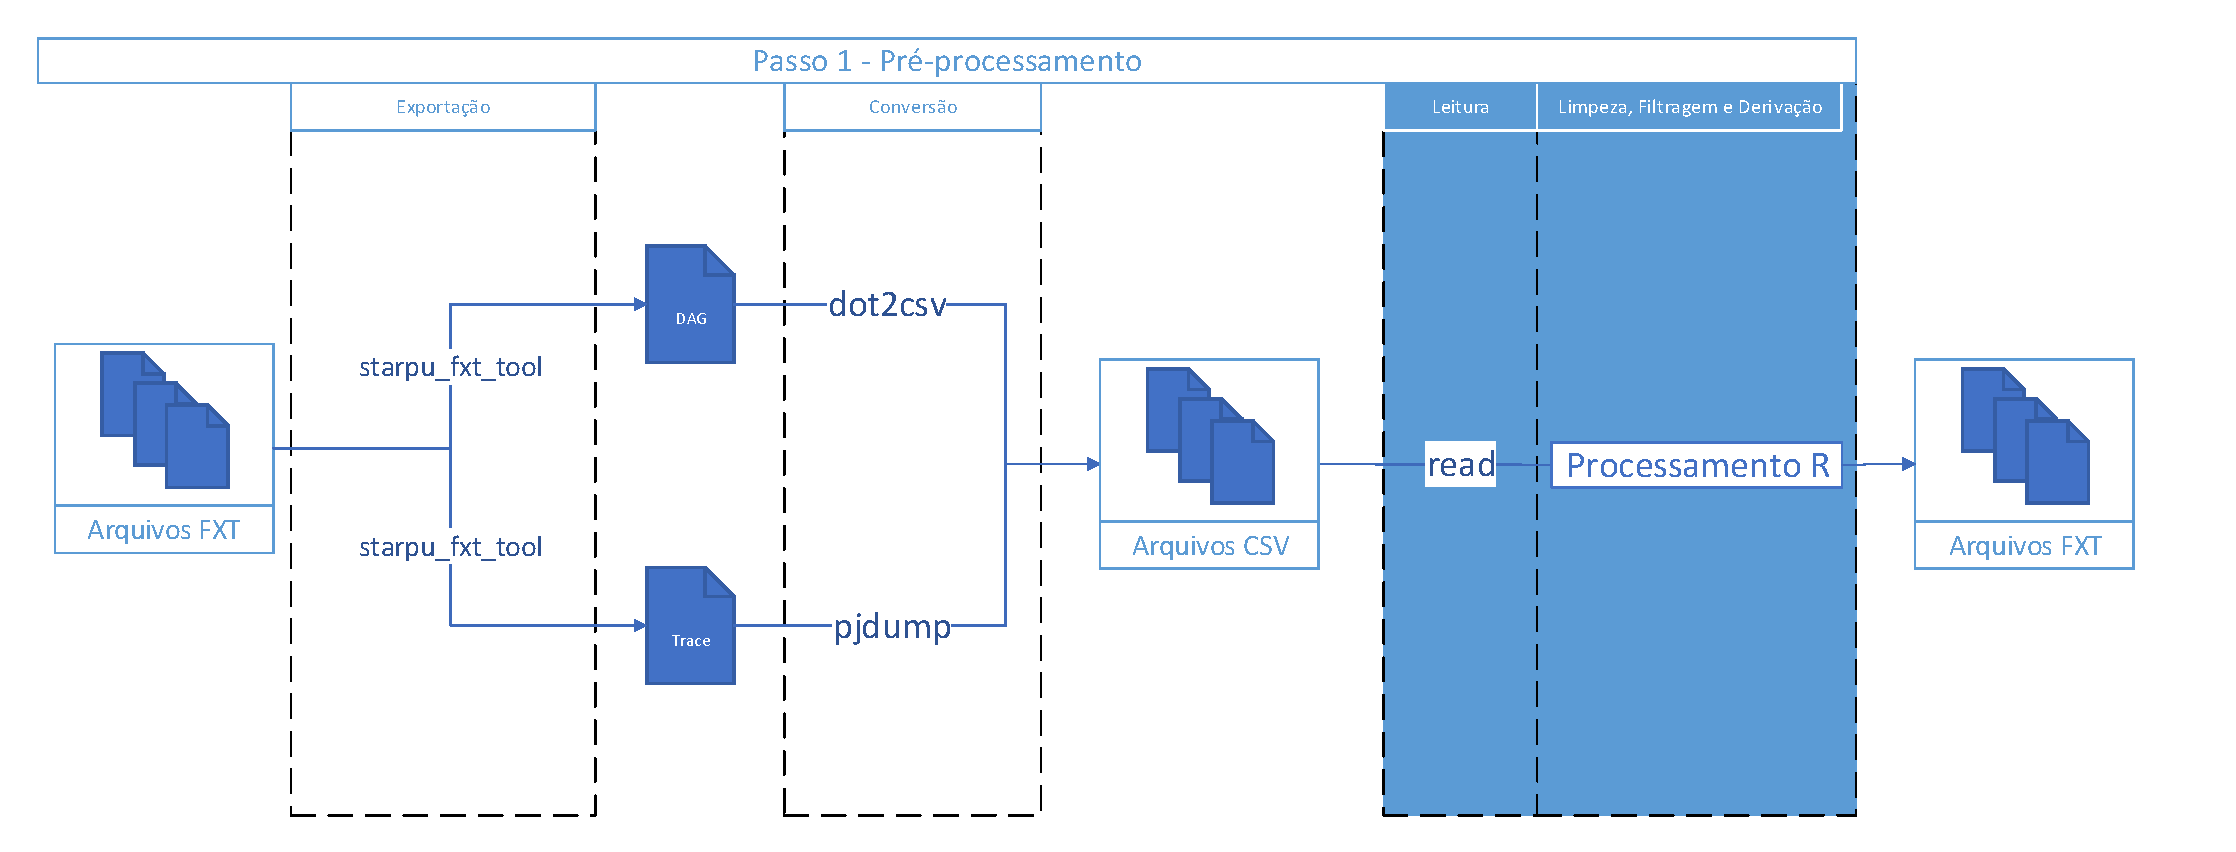
\includegraphics[width=1\textwidth]{./images/step1-simpler.pdf}}
 \legend{Etapas do passo de pré-processamento do StarVZ}
 \label{fig:starvz-steps}
\end{figure}


%%%%%%%%%%%%%%%%%%%%%%%%%%%%%%%%%%%%%%%%%%%%%%%%%%%%%%%%%%%%%%%%%%%%%%%%%%%%%%%%%%%%%
% METODOLOGIA
%
\chapter{Metodologia} \label{lbl:metodologia}

Primeiramente, serão realizados experimentos para identificar com precisão a quantidade de tempo
envolvida em cada uma das etapas do pré-processamento do \emph{framework} em sua implementação original. Isso se faz necessário
pois os tempos citados no trabalho de \citet{ref:starvz} são todos aproximações. Além disso, serão realizados experimentos com 
outras entradas, portanto, é coerente que tudo seja executado com os mesmos recursos.

Os CSVs de saída da etapa de conversão serão carregados no HDFS \cite{ref:hdfs} para leitura distribuída. A expectativa é que isso já traga algum ganho de desempenho, visto que a vazão de leitura de múltiplos discos é maior do que de apenas um. Em seguida, serão executadas as operações do passo de \emph{Limpeza, Filtragem e Derivação} de forma distribuída, utilizando o Spark \cite{ref:spark}.

Os arquivos \emph{Feather} resultantes do pré-processamento serão validados com uma execução do \emph{framework} original, para garantir que ambos geram a mesma saída. Após isso, serão realizados experimentos comparando ambas implementações para determinar se houve ganho de desempenho utilizando essa abordagem distribuída.

%%%%%%%%%%%%%%%%%%%%%%%%%%%%%%%%%%%%%%%%%%%%%%%%%%%%%%%%%%%%%%%%%%%%%%%%%%%%%%%%%%%%%
% CRONOGRAMA
%
\chapter{Cronograma} \label{lbl:cronog}

O cronograma deste trabalho se divide em 4 etapas:

\begin{itemize}
    \item Implementação - realizar modificações no código do \emph{framework};
    \item Experimentação - avaliar os resultados do que foi implementado;
    \item Pesquisa e Escrita - pesquisar trabalhos relacionados e escrever monografia;
    \item Apresentação - produzir apresentação de slides para a defesa.
\end{itemize}

\begin{table}[H]
    \centering
    \begin{tabular}{|p{1.8in}|p{0.5in}|p{0.5in}|p{0.5in}|p{0.5in}|} \hline 
Etapa & \multicolumn{4}{|p{2.0in}|}{Meses} \\ \hline 
 & Mai & Jun & Jul & Ago  \\ \hline 
Implementação & X & X &  &   \\ \hline 
Experimentação &  & X & X &   \\ \hline 
Pesquisa e Escrita & X & X & X & X  \\ \hline 
Apresentação &  &  & X & X  \\ \hline 
\end{tabular}
    \legend{Cronograma de execução do trabalho.}
    \label{tab:cronog}
\end{table}



%%%%%%%%%%%%%%%%%%%%%%%%%%%%%%%%%%%%%%%%%%%%%%%%%%%%%%%%%%%%%%%%%%%%%%%%%%%%%%%%%%%
% BIBLIOGRAFIA 
%%%%%%%%%%%%%%%%%%%%%%%%%%%%%%%%%%%%%%%%%%%%%%%%%%%%%%%%%%%%%%%%%%%%%%%%%%%%%%%%%%%
%
\bibliographystyle{abntex2-alf}
\bibliography{biblio} 

\end{document}
